\section{Introduction}
\label{introduction}


% state the learning objective
\par The aim of this laboratory assignment was to create an audio amplifier circuit. To do so, both the gain and the output stages were designed. This amplifier receives an audio maximum input of 10mV and connects to an 8 Ohm speaker. The source has an impedance of 100 Ohms and the circuit is supplied by a 12V Voltage DC source (vcc).
\par In the gain stage mentioned above, a NPN transistor and a common emitter amplifier with degeneration were used. It allows us to have a high $Z_{i}$ and a high $A_{V}$. Nevertheless, $Z_{o}$ is also very high, which consitutes a problem. Hence, this situation has to be adressed in the output stage. Consequently, in this second stage, it was used a common collecter amplifier and a PNP transistor. Not only does it allow to remain a high $A_{V}$ but it also reduces the value of $(Z_{o})$ significantly. Therefore, the gain is $\approx 1$, which is the desired result.

\par The quality of the audio amplifier is evaluated by the following expression:
\begin {equation}
	 MERIT = \frac{Voltage Gain*Bandwidth}{Cost*Lower Cut Off Frequency}   	
	\label{merit}
\end{equation}

The circuit is shown below.

\begin{figure}[ht] \centering
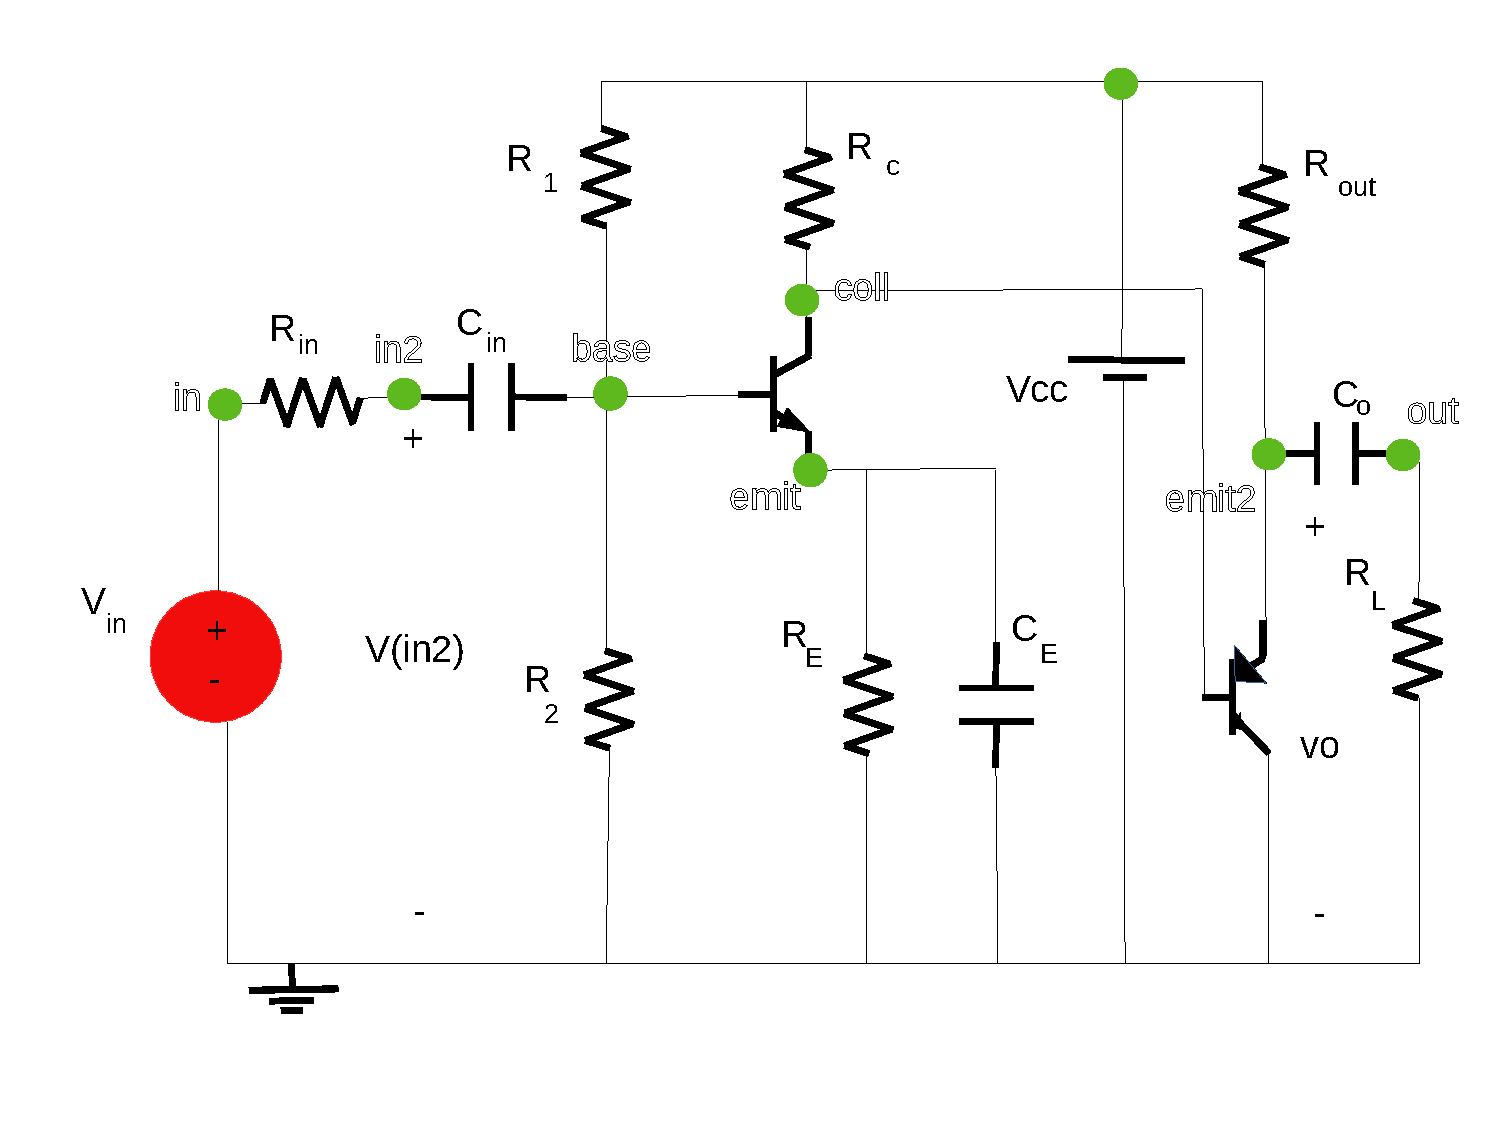
\includegraphics[width=0.8\linewidth]{lab4.pdf}
\caption{Circuit i analysis.}
\label{circuito todo}
\end{figure}
\par 


\newpage
